\section{Tool Development}
\label{Development}

The Automatic Translation tool comprises of a set of components such as the meta-models for UML Activity Diagram and Java, the Activity Diagram model editor, model to model transformations and model to text transformations. Each of these components is addressed in detail in this section, and is illustrated in Fig.~\ref{figure:overalltool}.

\begin{figure}[!h]
	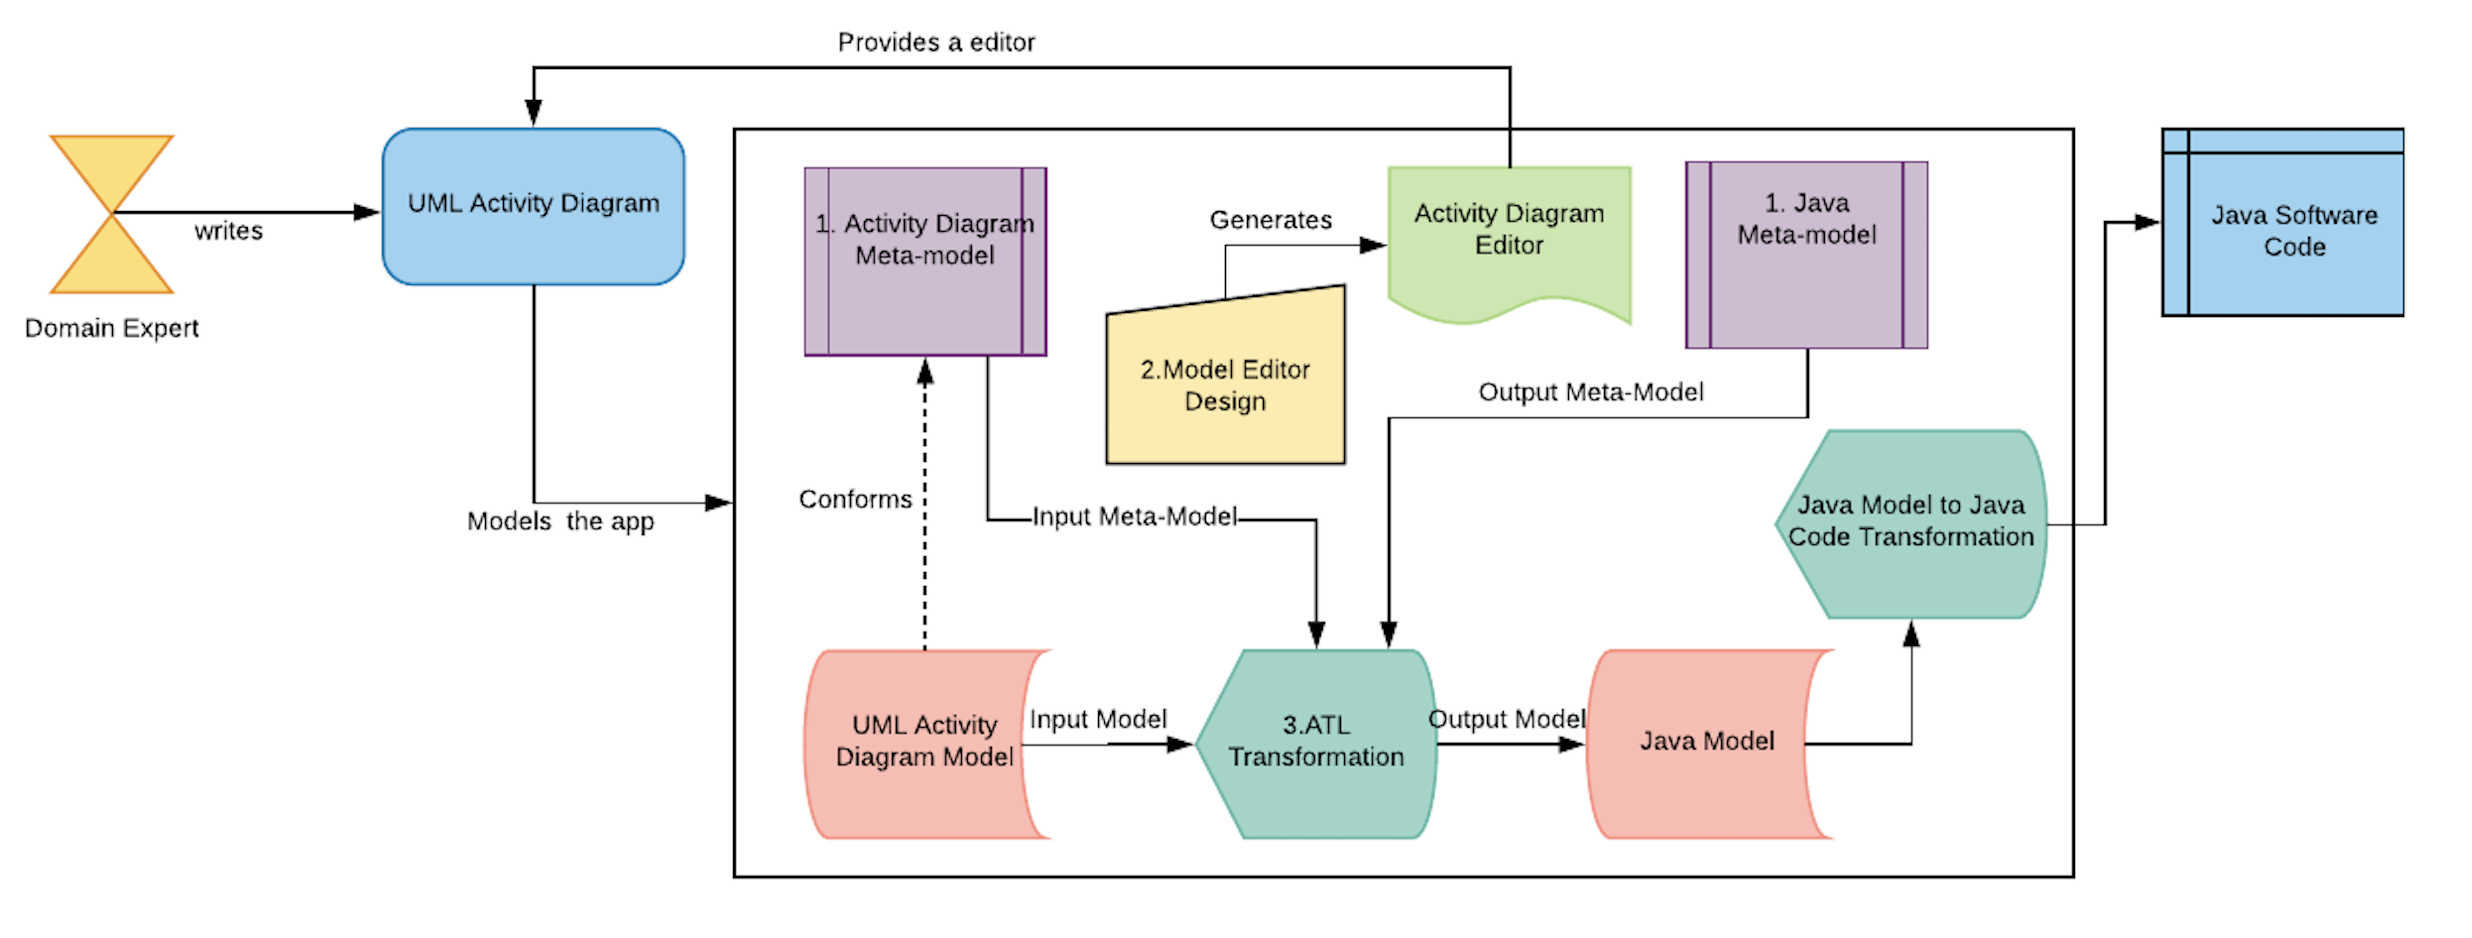
\includegraphics[width=\textwidth]{figs/Architecture_Proposed_Solution}
	\caption{Detailed View of the Architecture}
	\label{figure:overalltool}
\end{figure}

\subsection{Component 1: Meta-Model Design}
\label{Component1}
Component 1 represents the design and development of both the UML Activity Diagram meta-model and the Java meta-model \cite{perera2018thesis}. Meta-models for both Java and UML Activity diagrams are designed using the EMF Framework and Ecore Tools in Eclipse. The Activity Diagram meta-model in shown in Fig.~\ref{figure:ADMetaModel}. 

\begin{figure}[!h]
\centering
	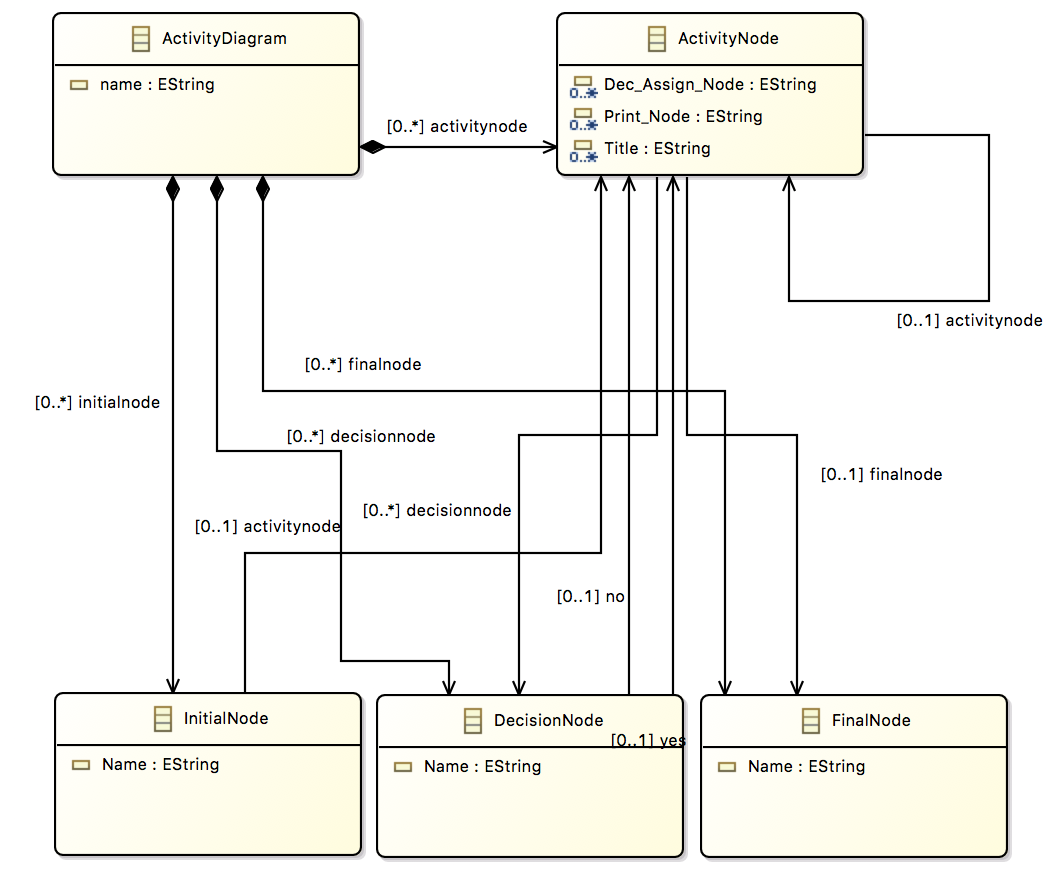
\includegraphics[width=0.8\textwidth]{figs/Activity_Diagram_Meta_Model}
	\caption{Activity Diagram Meta-Model}
	\label{figure:ADMetaModel}
\end{figure}

%The configuration of Figure \ref{figure:ADMetaModel} generates an Activity Diagram Model Instance based on a generic Smart Lighting System. This is shown in the figure below.

\begin{comment}
\begin{figure}[!h]
	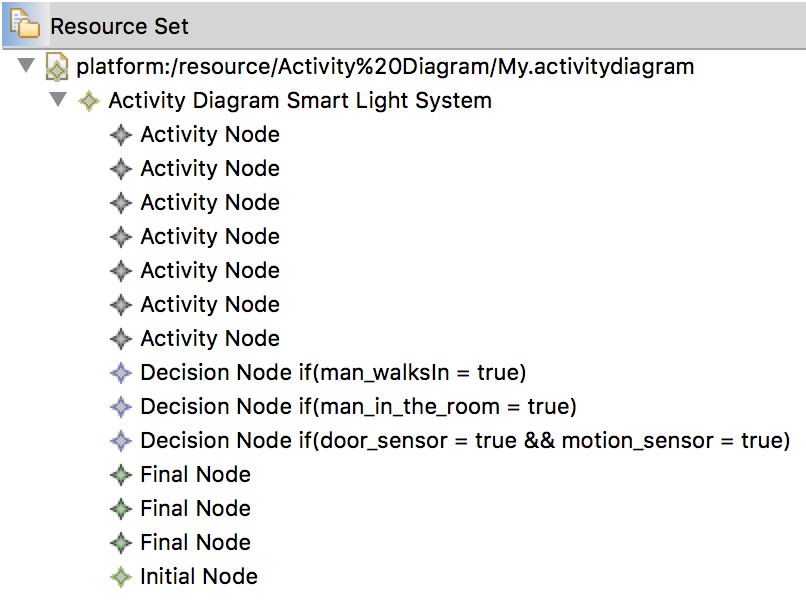
\includegraphics[width=\textwidth]{figs/Activity_Diagram_Model_Instance}
	\caption{Activity Diagram Model Instance (Smart Lighting System)}
	\label{figure:Activity_Diagram_Model_Instance}
\end{figure}
\end{comment}

\subsection{Component 2: Customized Activity Diagram Model Editor}
A customized model editor has been designed with the support of Sirius, an Eclipse plug-in. The model editor consists of a \textit{viewpoint} which supports the connection of the activity diagram meta-model and the model editor. A viewpoint in Sirius provides a set of representations, and in this case, the representation is called "\textbf{\textit{activitydiagram}}" which is synchronized with the activity diagram meta-model. The activation of this viewpoint allows creating and editing of the corresponding activity diagram in the activity diagram model editor \cite{perera2018thesis}. Fig.~\ref{figure:modeleditor} shows a screenshot of the model editor in which a smart lighting system has been modelled.

\begin{figure}[!h]
	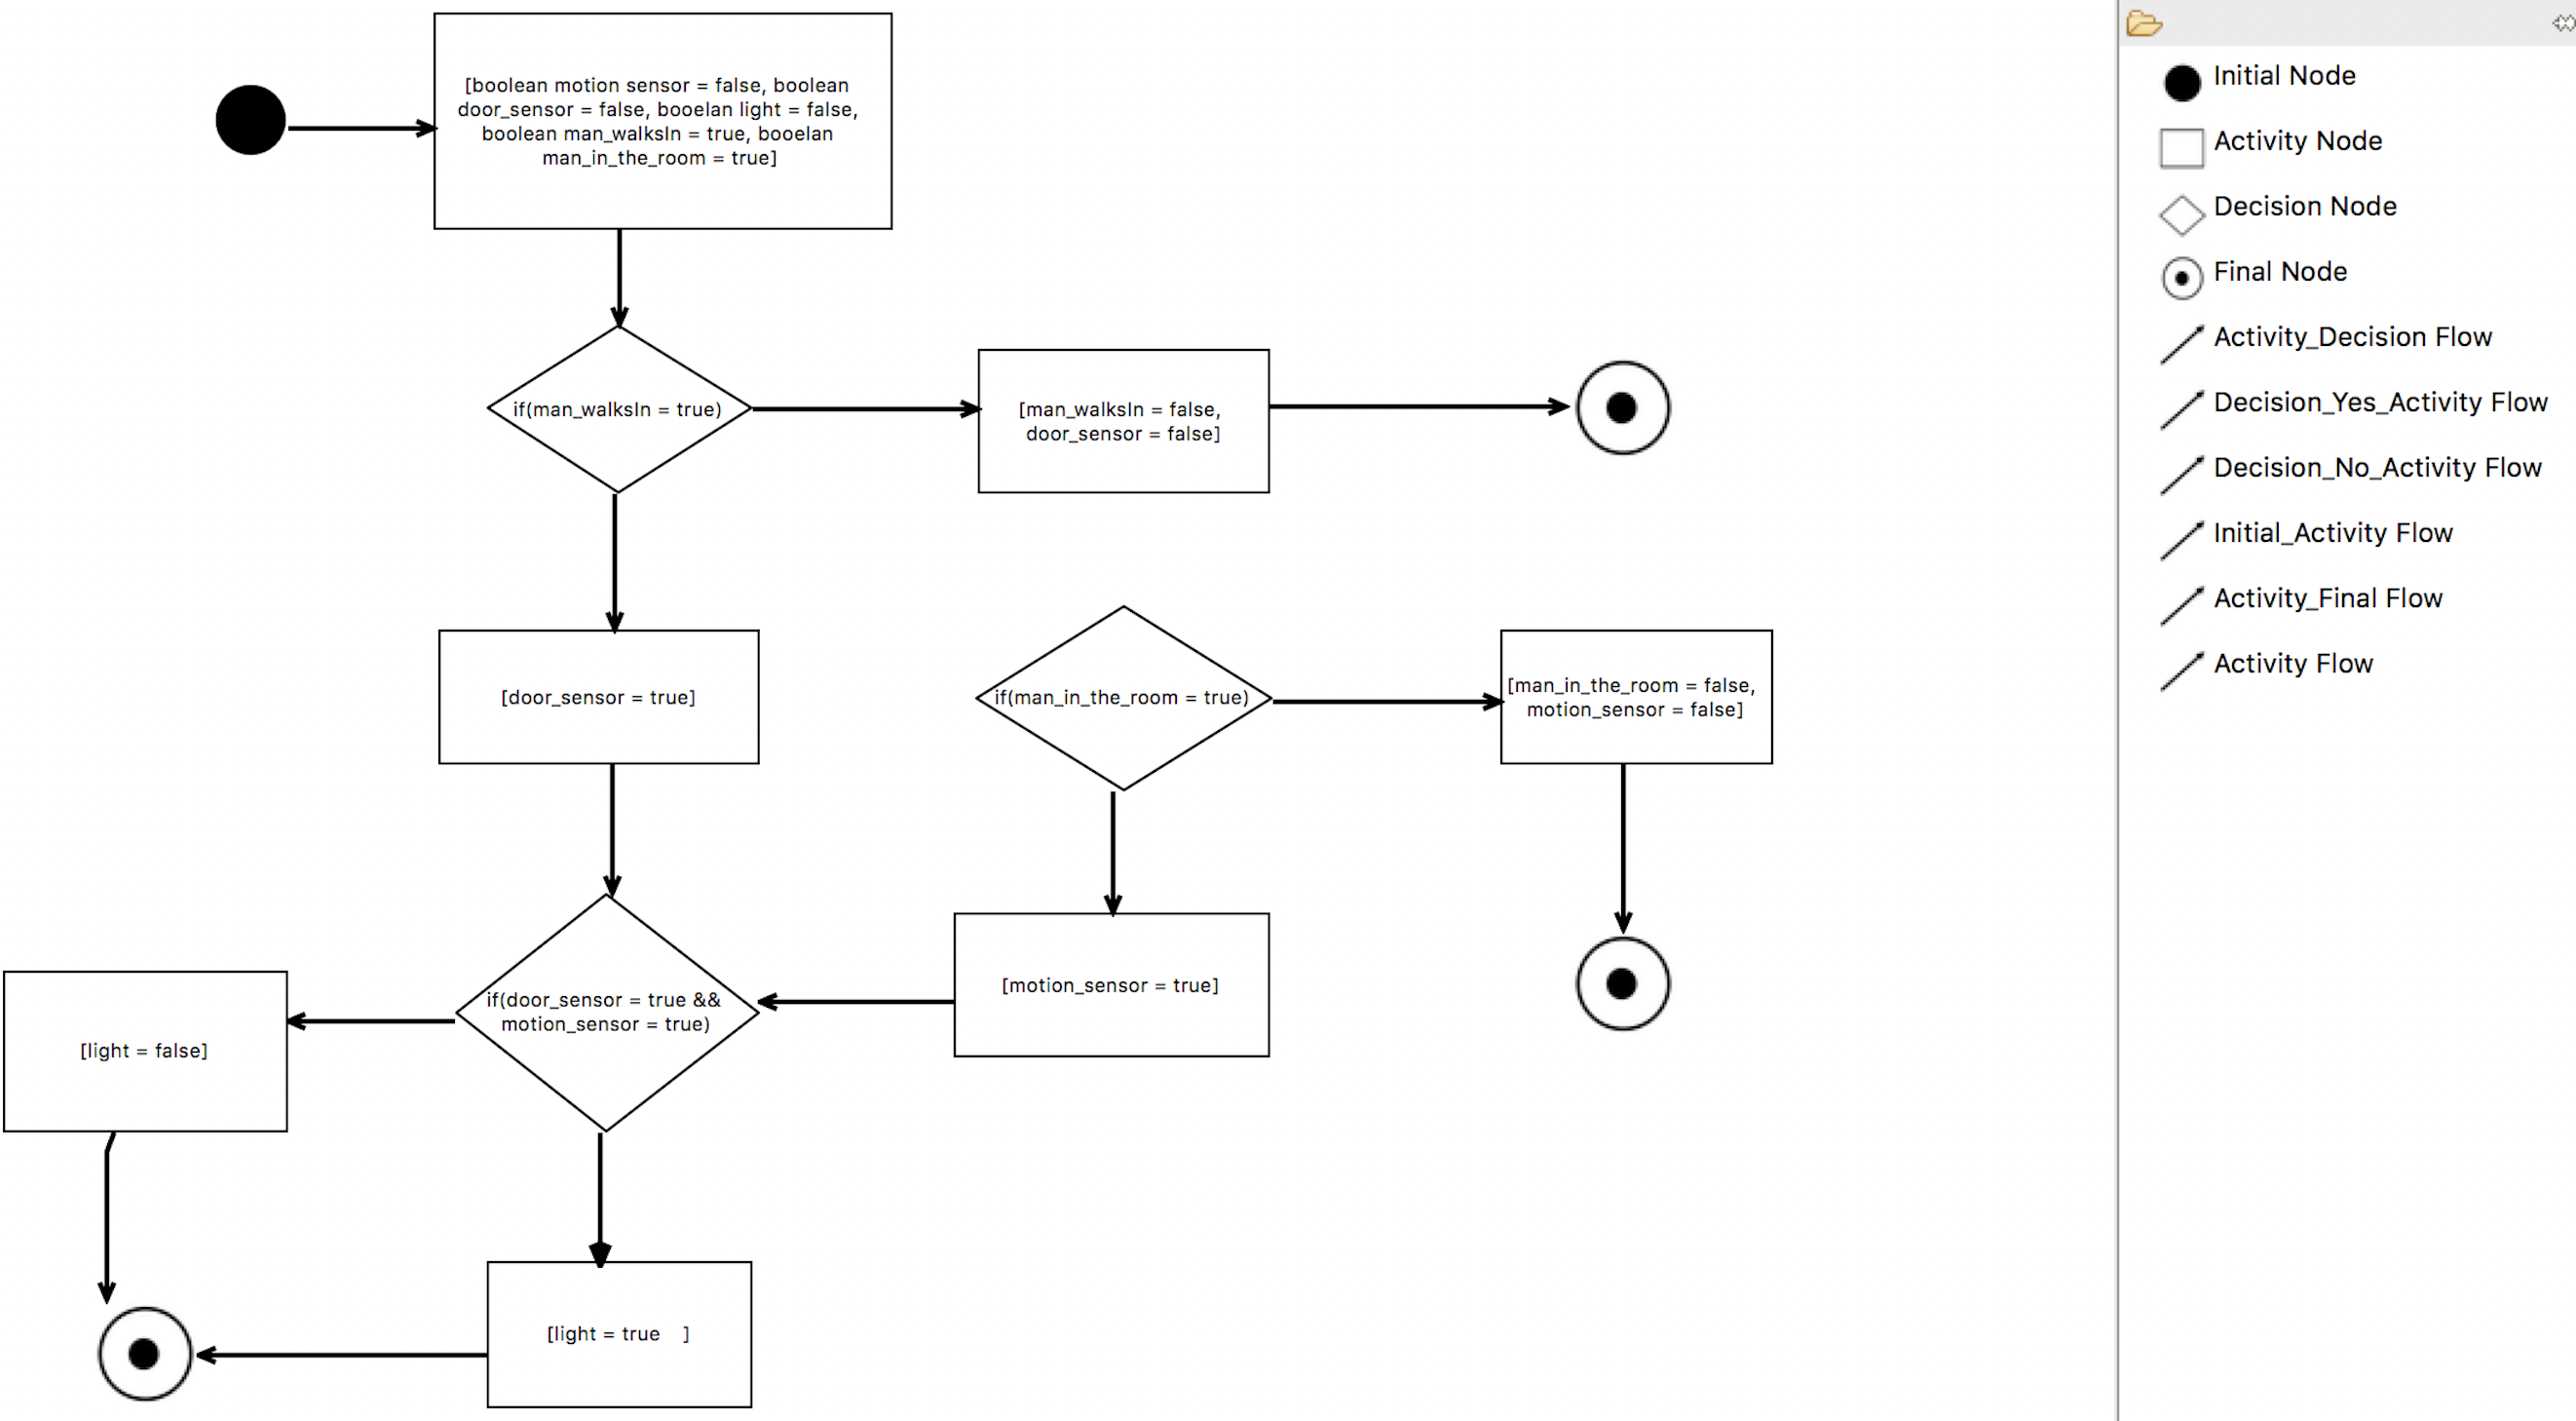
\includegraphics[width=\textwidth]{figs/Activity_Diagram_Model_Editor}
	\caption{Activity Diagram Model Editor depicting a Smart Light System}
	\label{figure:modeleditor}
\end{figure}


\subsection{Component 3: Model-to-Model Transformation}
\label{Component 3: Model-to-Model Transformation}

This technique is used to map the Activity Diagram model to the Java model which eventually supports the generation of software code. ATL is chosen to map and transform models since it is supported by Eclipse which in turn may support the design and development in term of compatibility. The mapping of Activity Diagram Meta-Model and Java Meta-Model with Activity Diagram Model Instance used as the input model (Fig.~\ref{figure:modeleditor}) is shown in Fig.~\ref{figure:ATL_Mapping_Approach}. This configuration process supports the generation of the corresponding Java Model Instance which is later translated into runnable code.

\begin{figure}[!h]
\centering
	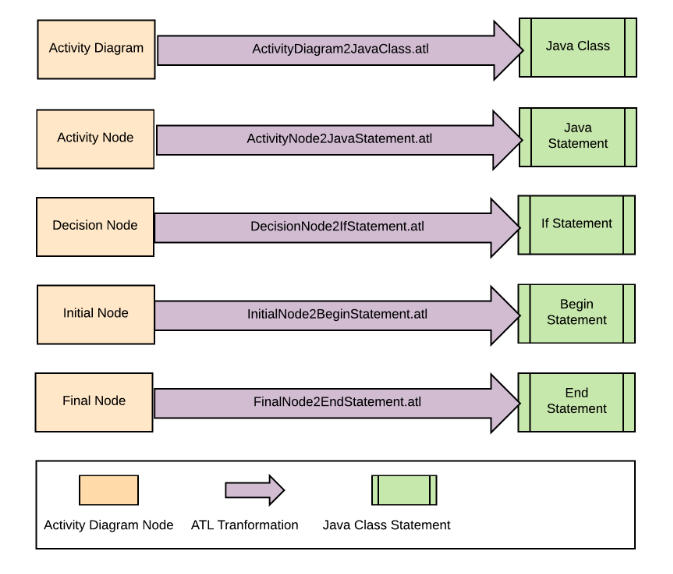
\includegraphics[width=0.6\textwidth]{figs/ATL_Mapping_Approach}
	\caption{ATL Mapping Approach}
	\label{figure:ATL_Mapping_Approach}
\end{figure}



\subsection{Component 4: Model-to-Text Transformation}

The Model-to-Text transformation method is used in the tool to support code generation from the model generated during the mode-to-model transformation. In order to generate Java Code from the model instance which is in XMI format, the file is read using a Java program line by line where each line comprises of a tag name which corresponds with the type of the statements in the code model. Every line is written to a Java file. The Java code generated from the smart lighting system model illustrated in Fig.~\ref{figure:modeleditor} is shown in Fig.~\ref{figure:Generated_Java_Code}.

\begin{figure}[!h]
	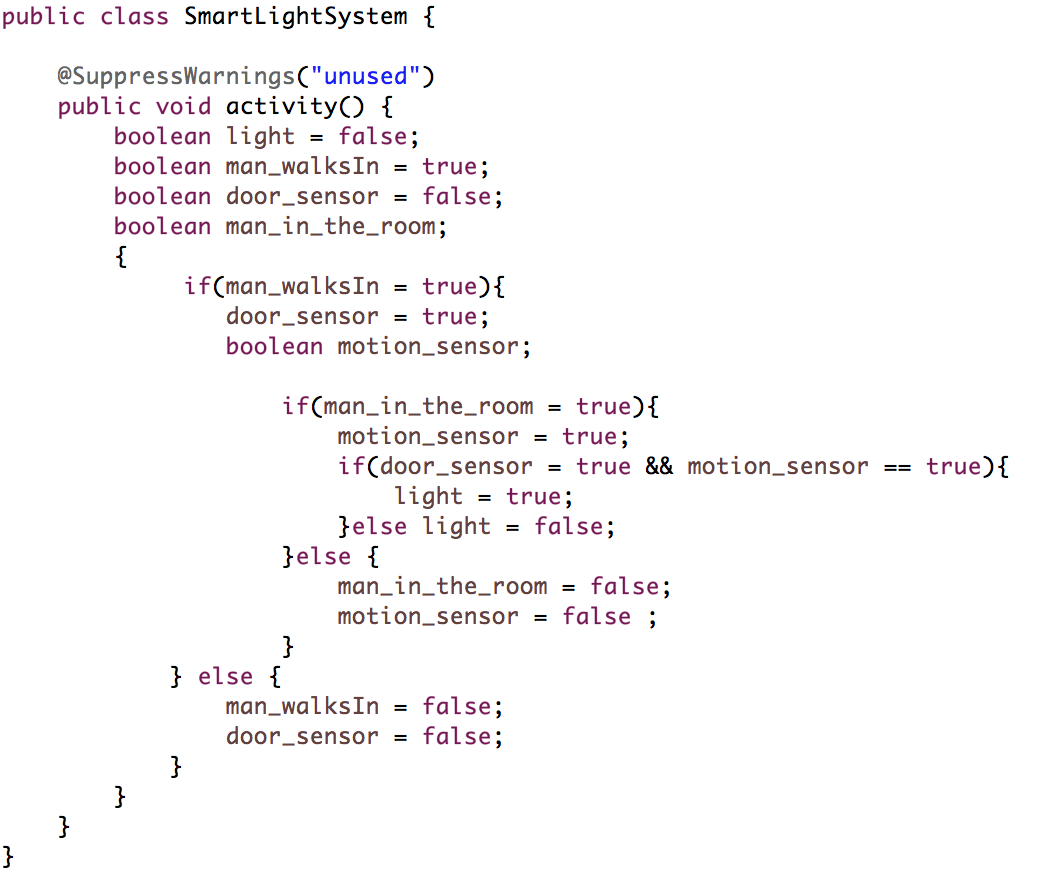
\includegraphics[width=\textwidth]{figs/Generated_Java_Code}
	\caption{Generated Java Code}
	\label{figure:Generated_Java_Code}
\end{figure}


